\chapter{Diseño e Implementación} % Main chapter title

\label{Chapter3} % Change X to a consecutive number; for referencing this chapter elsewhere, use \ref{ChapterX}
\definecolor{mygreen}{rgb}{0,0.6,0}
\definecolor{mygray}{rgb}{0.5,0.5,0.5}
\definecolor{mymauve}{rgb}{0.58,0,0.82}

%----------------------------------------------------------------------------------------

La idea de este capítulo es explicar los criterios utilizados en el desarrollo del producto y justificar las decisiones de diseño; así como también explicar el detalle de la implementación de los distintos aspectos del producto.

\section{Hardware}
\label{section:hardware}

En el contexto del presente trabajo, se desarrolló un prototipo funcional del producto final. Este prototipo presenta las mismas funciones que el equipo final pero no se ajusta a los lineamientos estéticos y mecánicos que si deberá cumplir el producto. Es por esto que el prototipo diseñado tiene dimensiones mucho más grandes que las que tendrá, lo cual facilitó las mediciones y pruebas que se debieron realizar para comprobar el correcto funcionamiento tanto del hardware como del firmware. 

En la Figura \ref{fig:prototipo} puede verse una fotografía del prototipo. En la misma se puede apreciar el PCB diseñado y las dos conexiones principales: a la izquierda del gabinete la conexión a la línea eléctrica y a la derecha la conexión a la carga eléctrica. La placa fue colocada dentro de un gabinete que por supuesto no tiene relación alguna con el gabinete que finalmente se utilizará. Simplemente cumple la función de facilitar la manipulación del prototipo.

\begin{figure}[h]
	\centering
	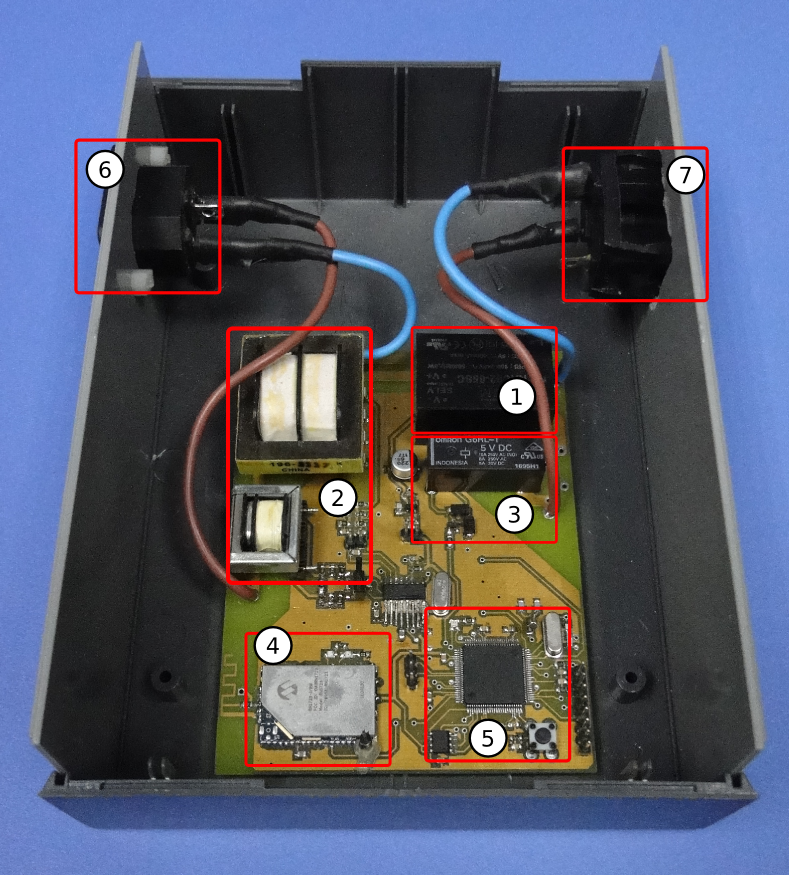
\includegraphics[width=11cm]{./Figures/3_1_prototipo_1.png}
	\caption{Prototipo funcional del Smart Plug. 1 - Fuente de alimentación. 2 - Adaptación de las señales de línea. 3 - Control de la carga. 4 - Módulo WiFi. 5 - Microcontrolador, led bicolor, pulsador y memoria EEPROM. 6 - Conexión a la línea eléctrica. 7 - Conexión a la carga.}
	\label{fig:prototipo}
\end{figure}

Los bloques mencionados en la Figura \ref{fig:prototipo} son explicados en las Subsecciones \ref{subsec:esquematico_general} y \ref{subsec:detalles_hardware}.

A pesar de ser un prototipo funcional, el hardware se diseño pensando en las caracteríticas finales que tendrá el producto. Por lo tanto se debieron definir las especificaciones deseadas para el equipo:

\begin{itemize}
\item Tensión máxima de operación: 240VAC
\item Corriente máxima de operación: 5A
\end{itemize}

Para una tensión de operación de 220VAC, la máxima potencia que se puede conectar es de 1100W. Para un primer producto se buscó cubrir la automatización de aparatos eléctricos de baja potencia como lámparas, ventiladores, electrodomésticos pequeños, televisores, etc. El manejo de equipos de mayor potencia como aires acondicionados, estufas eléctricas, hornos eléctricos, etc, será cubierto en un futuro cuando se modifique el hardware para soportar una mayor corriente, generando así un nuevo producto.



\subsection{Esquemático general}
\label{subsec:esquematico_general}

En la Figura \ref{fig:hardware_diagrama_bloques} pueden verse los principales bloques funcionales del prototipo.

\begin{figure}[h]
	\centering
	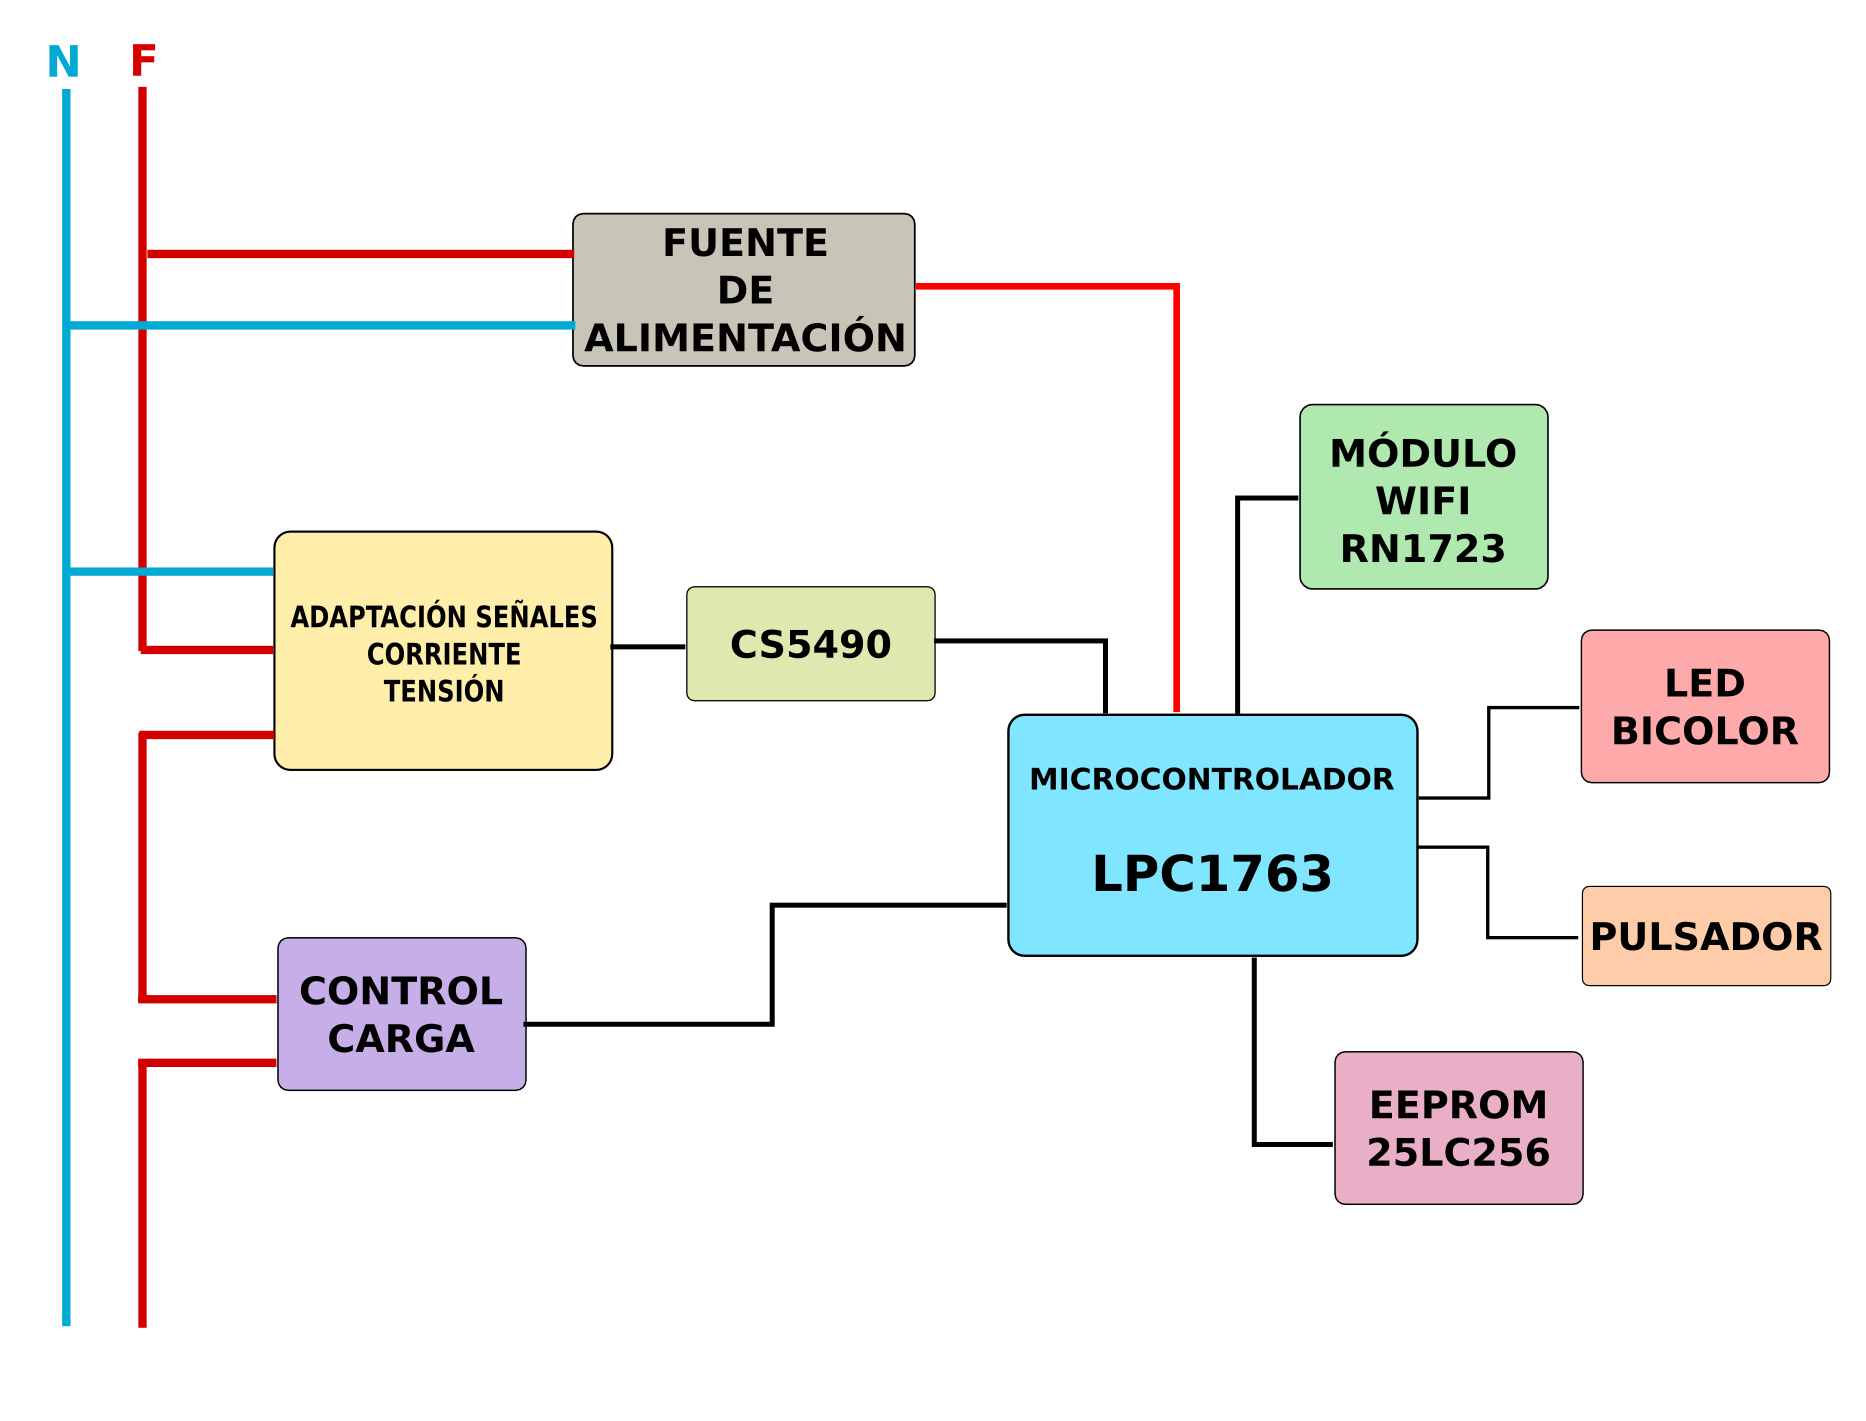
\includegraphics[width=12cm]{./Figures/3_1_1_diagrama_bloques_hardware.png}
	\caption{Diagrama en bloques del hardware del prototipo funcional.}
	\label{fig:hardware_diagrama_bloques}
\end{figure}

A continuación se describe brévemente cada uno de los módulos. Una explicación más detallada de cada uno se encuentra en la Subsección \ref{subsec:detalles_hardware}:

\begin{itemize}
\item Fuente de alimentación. La alimentación del equipo es obtenida de la misma línea eléctrica a la que está conectado el dispositivo. Debe generar dos niveles de tensión, 5V y 3,3V y debe ser capaz de entregar soportar el consumo especialmente del módulo WiFi.
\item Adaptación de las señales de corriente y tensión. Este bloque se encarga de adaptar la señal de tensión de la línea y la señal de la corriente consumida por el aparato eléctrico a los niveles que requiere el front-end analógico CS5490. La adaptación se realiza mediante transformadores para lograr una completa aislación de la línea.
\item Front-end analógico CS5490. Es el circuito integrado encargado de tomar las señales de la línea y generar las mediciones eléctricas de interés: tensión eficaz, corriente eficaz, frecuencia de línea, factor de potencia, energía consumida, etc.
\item Control de la carga. La conmutación de la carga se realiza mediante un relay mecánico.
\item Módulo WiFi RN1723. Es el módulo encargado de permitir la comunicación entre el Smart Plug y la aplicación móvil. Básicamente se encarga de esperar conexiones TCP y enviar las respuestas requeridas al socket del que provino el comando.
\item Microcontrolador LPC1763. Es el encargado de implementar la lógica del Smart Plug. 
\item Memoria EEPROM. Es la encargada de retener información de configuración del Smart Plug y las mediciones diarias de potencia y energía.
\item Led bicolor. Es un led rojo y verde encargado de realizar las señalizaciones acerca del funcionamiento del equipo. En la Subsección \ref{sec:validacion_firmware} se describe el significado de las distintas señalizaciones.
\item Pulsador. Mediante el pulsador se inician loas procesos destinados a incorporar el Smart Plug a la red WiFi de la casa.
\end{itemize}

\subsection{Descripción de los módulos de hardware}
\label{subsec:detalles_hardware}

En este apartado de la memoria se describen las decisiones de diseño asociadas a los módulos de hardware. Los fragmentos de esquemático que a continuación se muestran surgen del archivo \textit{SmartPlug\_v1.0} en \citep{repo_hardware}.

\subsubsection{Fuente de alimentación}

El esquemático de la fuente del Smart Plug puede verse en la Figura \ref{fig:pcb_fuente}. Esta fuente de alimentación se conecta a la misma línea eléctrica que es medida por el front-end analógico. A partir de la tensión de 220VAC genera una tensión de 5V y 3,3V. Para lograr los 5V se utiliza una fuente switching con montaje para PCB VSK-S2-5U la cual puede entregar hasta 400mA. Esta fuente permite generar una tensión estable manteniendo un empaquetado de reducido tamaño (34 x 22 x 18 mm). 

\begin{figure}[h]
	\centering
	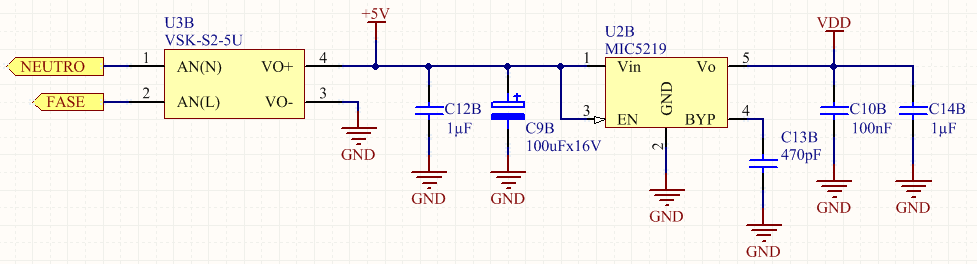
\includegraphics[width=14cm]{./Figures/3_1_2_pcb_fuente.png}
	\caption{Esquemático de la fuente de alimentación.}
	\label{fig:pcb_fuente}
\end{figure}


Se debe aclarar que esta switching fuente fue elegida para el prototipo funcional. En la versión final del equipo se utilizará una fuente switching AC-DC de similares características diseñada dentro de la empresa, debido a que tanto el tamaño del empaquetado de la fuente como su costo (U\$s 13,25 por unidad al momento de escribir la memoria) son prohibitivos para incluir esta fuente en el diseño final.

En cuanto al regular de 3,3V se eligió un componente que puede entrgar hasta 500mA. El requerimiento de corriente tanto de la fuente switching como del regulador de 3,3V surge del consumo especialmente del módulo WiFi RN1723, el cual puede consumir hasta 250mA.


\subsubsection{Adaptación de las señales de tensión y corriente}

En la Figura \ref{fig:pcb_adaptacion} puede verse la sección del esquemático relacionada con la adaptación de las señales de tensión y de corriente del dispositivo. Para poder obtener las mediciones eléctricas y el consumo de la carga conectada al Smart Plug es necesario adaptar las señales de tensión de línea y de la corriente consumida por la carga a los niveles soportados por el front-end analógico.

\begin{figure}[h]
	\centering
	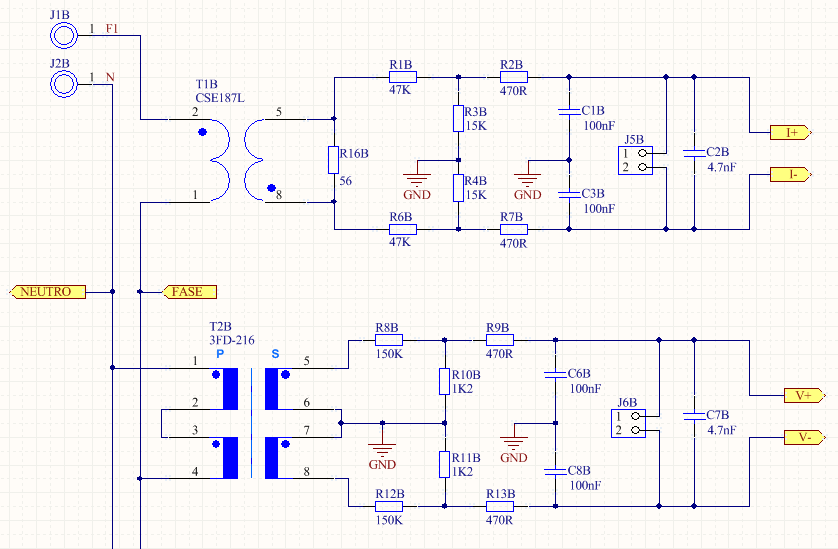
\includegraphics[width=14cm]{./Figures/3_1_2_pcb_adaptacion.png}
	\caption{Esquemático de la etapa de adaptación de las señales de tensión y corriente de la línea eléctrica.}
	\label{fig:pcb_adaptacion}
\end{figure}

De acuerdo a la hoja de datos del front-end elegido para este proyecto (CS5490) tanto la señal de corriente como la de tensión no deben superar los 250mV de pico en las entradas diferenciales del circuito integrado. Para lograr esto, primero se debe definir la tensión y la corriente máxima que debe medir el Smart Plug. En el caso concreto de este proyecto, y como ya fue mencionado, estos valores son: tensión máxima - 240VAC, corriente máxima - 5A.

Definidos estos valores, se eligió aislar el resto del circuito de la línea eléctrica tomando las señales de tensión y corriente mediante transformadores. Al igual que sucedió con la elección de la fuente switching, esta decisión fue exclusivamente para el desarrollo del prototipo funcional, ya que en la versión final será conveniente reemplazar el transformador de tensión por divisores resistivos y el transformador de corriente por un shunt. Ambos cambios van a permitir reducir el tamaño del producto final y su costo.

Luego de los transformadores hay divisores resistivos dispuestos en forma diferencial para reducir la tensión a los valores tolerados por el CS5409. Finalmente hay filtros pasa-bajo con un a frecuencia de corte de 3,3kHz.

Con los valores elegidos de relación de transformación y divisores resistivos, los valores máximos soportados por el equipo resultan:

\begin{itemize}
\item Tensión máxima soportada por el hardware: 320VAC.
\item Corriente máxima soportada por el hardware: 6,5A.
\end{itemize}

Ambos valores se encuentran por encima de los valores máximos informados al usuario.


\subsubsection{Front-end analógico}

Luego de adaptar las señales de tensión y de corriente, las mismas deben ser medidas por un front-end analógico que se encargará de generar los parámetros de interés para la aplicación: tensión y corriente eficaz, frecuencia de línea, potencia activa, factor de potencia, energía consumida, etc. En la Figura \ref{fig:pcb_medicion_energia} puede verse l circuito asociado al front-end elegido, el CS5490.

\begin{figure}[h]
	\centering
	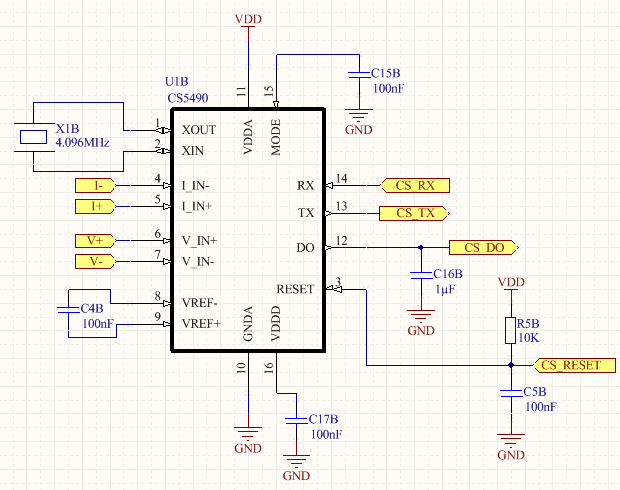
\includegraphics[width=14cm]{./Figures/3_1_2_pcb_medicion_energia.png}
	\caption{Esquemático del front-end analógico encargado de medir los parámetros eléctricos.}
	\label{fig:pcb_medicion_energia}
\end{figure}

A parte de los componentes relacionados con la adaptación de las señales de línea, este circuito integrado  no necesita de una gran cantidad de componentes adicionales, salvo algunos capacitores y un cristal de 4,096Mhz con el cual va generar la base de tiempo interna para realizar las mediciones y cálculos.

La comunicación es sencilla, a través de comandos enviados por una UART. Con estos comandos se van poder conocer casi todas las mediciones que calcula el CS5490. La única medición que no puede ser conocida a través de la lectura de un registro es la energía consumida. Esta es informada mediante pulsos a través del pin \textit{DO}. Se debe configurar la constante del medidor en el CS5490, es decir la cantidad de pulsos a los que equivale un kilowatt-hora.


\subsubsection{Control de la carga}

La conmutación de la carga está a cargo de un relay mecánico. En la Figura \ref{fig:pcb_control_carga} puede verse que la fase de la línea eléctrica se conecta entre los contactos \textit{común} y \textit{normal cerrado} del relay para que, en caso de ocurrir un desperfecto con el Smart Plug, la carga pueda seguir funcionando.

\begin{figure}[h]
	\centering
	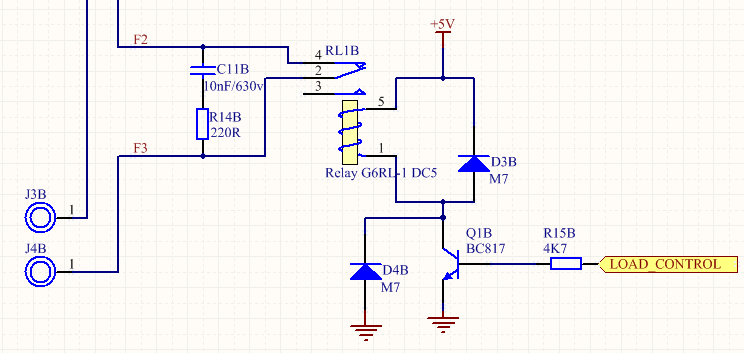
\includegraphics[width=10cm]{./Figures/3_1_2_pcb_control_carga.png}
	\caption{Esquemático del control de la carga eléctrica mediante un relay mecánico.}
	\label{fig:pcb_control_carga}
\end{figure}

Para funcionar, la bobina del relay requiere de una tensión de 5V y los contactos soportan una corriente máxima de 8A con 250VAC, valor que satisface sobradamente las especificaciones propuestas para el Smart Plug.

\subsubsection{Módulo WiFi}

El módulo elegido es el RN1723, el cual prácticamente no requiere de componentes adicionales y se comunica con el microcontrolador mediante una UART.

Para la antena del módulo se eligió una antena impresa en el PCB de acuerdo a las especificaciones de la hoja de datos del módulo.

Al momento de comenzar con el proyecto y elegir los componentes, este módulo resultaba una opción atractiva, que proveía las funcionalidades especificadas en los requerimientos del producto a un precio aceptable. Además se decidió elegir este módulo ya que es comercializado por Microchip, marca que es ampliamente usada por los productos de X-28 Alarmas, lo cual lleva a la posibilidad de obtener precios muy competitivos con los distribuidores.

\section{Firmware}

\subsection{Arquitectura del firmware}

El firmware embebido en el Smart Plug se escribió utilizando FreeOSEK como sistema operativo de tiempo real. De esta forma, en la Figura \ref{fig:firmware_esquema_tareas} pueden verse las tareas que se crearon y la interacción que entre estas.

Básicamente, las características del firmware surgen de los requerimientos enumerados en la Sección \ref{sec:requerimientos} y son:

\begin{itemize}
\item Iniciar el proceso de WPS o configurarse en modo punto de acceso (AP) cuando se presiona el pulsador presente en la placa.
\item Mostrar el estado del dispositivo a través del led bicolor.
\item Escuchar las conexiones TCP que provengan de las aplicaciones móviles y generar las respuestas adecuadas.
\item Guardar de forma no volátil (en la memoria EEPROM) la potencia activa promedio y energía consumida de cada hora del día. En la EEPROM se guarda la información de los últimos 7 días.
\item  Sincronizar la hora del Smart Plug con un servidor NTP y gestionar el encendido y apagado de la carga de acuerdo a la programación horaria configurada.
\end{itemize}

\begin{figure}[h]
	\centering
	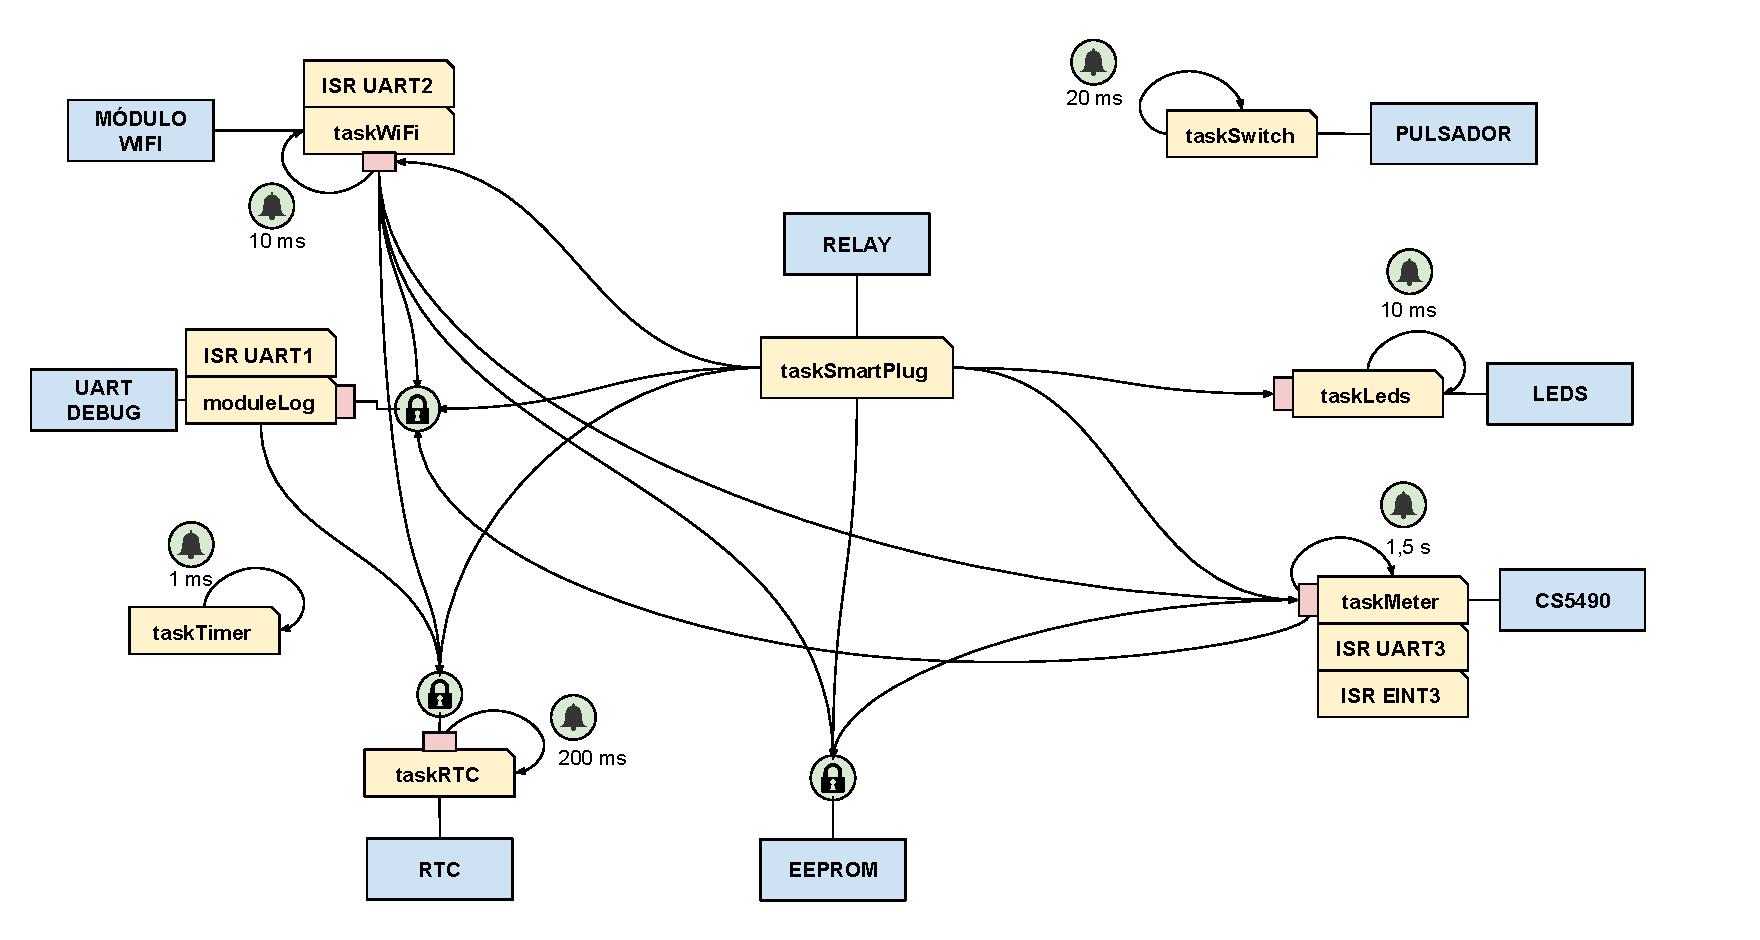
\includegraphics[width=16cm]{./Figures/3_2_1_firmware_esquema_tareas.pdf}
	\caption{Esquema de las tareas y recursos utilizados en el firmware.}
	\label{fig:firmware_esquema_tareas}
\end{figure}

A continuación se describe cada una de las tareas:

\begin{itemize}
\item taskSmartPlug. Es la tarea principal del Smart Plug. Se encarga de implementar la lógica del dispositivo. Se encarga de recibir los eventos generados por el resto de las tareas y realizar acciones en base a los mismos. Se va a bloquear esperando que ocurra alguno de los eventos. 

De taskWiFi obtiene los eventos relacionados con la conexión a la red WiFi y las conexiones TCP. Además le indica cuando tiene que iniciar un proceso de WPS o configurarse como punto de acceso.

A taskLeds le indica la señalización que debe realizar de acuerdo al evento recibido. En la Tabla \ref{tab:senializacion_leds} puede verse un resumen de todas las posibles señalizaciones.


De taskMeter obtiene las últimas mediciones para guardarlas de forma no volátil en la memoria EEPROM e ir generando un registro de potencia activa y energía consumida por hora de los últimos 7 días.

Además se encarga de manejar el relay que conmuta la carga eléctrica. El encendido o apagado de la misma se va a determinar a partir de la programación horaria (si está configurada) y de los comandos de encendido y apagado que envíe la aplicación móvil.

\item taskSwitch. Gestiona el pulsador de tipo tact switch que se encuentra en el PCB. Realiza el anti-rebote y genera los eventos cuando es presionado. Va a generar un evento cuando se suelte el pulsador (lo cual inicia el proceso de WPS en el módulo WiFi) y otro cuando se mantenga presionado por más de 5 segundos (lo cual configura al módulo WiFi como un punto de acceso). 

Es una tarea que se ejecuta cada 20ms mediante una alarma de FreeOSEK.


\item taskLeds. Se encarga de realizar las señalizaciones indicadas por otras tareas. Las señalizaciones se forman a partir de un led bicolor (rojo y verde), tanto encendiéndolos, apagándolos o haciéndolos destellar a distintas frecuencias.
Es una tarea periódica que se ejecuta cada 10ms, mediante una alarma de FreeOSEK, para actualizar los leds.


\item taskRTC. Se encarga de configurar y acceder al RTC interno del microcontrolador. Es la tarea que genera los eventos para indicar el paso de un minuto, una hora o un día, los cuales son utilizados por taskSmartPlug para registrar las mediciones de potencia activa y energía consumida por hora.

\item taskWiFi. Se encarga de recibir las conexiones desde la aplicación móvil. Interacciona con taskMeter para requerir las últimas mediciones de acuerdo a lo solicitado por la aplicación móvil.

También consulta la memoria EEPROM para leer o modificar los parámetros de configuración del Smart Plug y para enviarle a la aplicación móvil las mediciones históricas de potencia activa y energía consumida.

Cuando se inicia la tarea se conecta con un servidor NTP para obtener la fecha y hora. Estos parámetros son enviados a la tarea taskRTC para que configure el RTC interno del microcontrolador.

La comunicación con el módulo es a través de una UART y tanto la recepción como la transmisión se realizan a través de la interrupción de este periférico. La tarea es periódica, cada 10ms para controlar los mensajes que llegan desde el módulo RN1723  de forma asincrónica.

\item taskMeter. Se encarga de obtener periódicamente las mediciones del front-end analógico CS5490. Además acumula los pulsos generados por el mismo integrado para llevar un registro de la energía consumida por la carga.

Al iniciar la tarea, se encarga de configurar el CS5490 para que funcione de acuerdo a lo especificado. Este proceso incluye:

\begin{itemize}
\item Configurar la constante del meidor. Es la cantidad de pulsos a los que va a equivaler un kilowatt-hora. Para este proyecto se eligió una constante de 5000 pulsos/kWh. Esta constante no es configurada directamente en el CS5490, sino que se deben escribir algunos registros del integrado para lograr que genere 5000 pulsos por kWh. El proceso para lograr esto está explica en la Sección 5.5 de \citep{datasheet_CS5490}.
\item Configurar la tensión y corriente máxima de operación, ya que las mediciones van a ser calculadas a partir de estos parámetros.
\item Cargar los valores de calibración. Para lograr los valores de error relativo en el canal de tensión y de corriente que informa la hoja de datos es necesario realizar un proceso de calibración del equipo. Básicamente este proceso consta de dos etapas: calibración de \textit{offset} de continua y calibración de ganancia. Para el primero se deben cortocircuitar las entradas diferenciales del canal de tensión y de corriente y comenzar el proceso. Para la calibración de ganancia, en el caso de la tensión, se debe generar la tensión máxima que puede medir el Smart Plug y comenzar el proceso de calibración. Para el caso de la corriente, se puede usar una corriente menor a la máxima del Smar Plug que debe ser indicada al CS5490 antes de comenzar con la calibración.
Este proceso se encuentra detalladamente explicado en la Sección 7.1 de \citep{datasheet_CS5490}.

En el contexto del presente trabajo el proceso de calibración no se incluyó. Los valores de calibración se calcularon y luego se ajustaron manualmente. En la Sección \ref{sec:trabajo_futuro} se propondrá una posible forma de implementar la etapa de calibración en el proceso de fabricación del producto final.
\end{itemize}

La comunicación con el CS5490 se realiza a través de una UART y tanto la recepción como la transmisión se realizan a través de la interrupción de este periférico. Además se utiliza otra interrupción, encargada de detectar los pulsos generados por el CS5490 apra indicar la energía consumida.
Es una tarea periódica.

\item moduleLog. Es la tarea encargada de enviar información de la actividad de la aplicación a través de mensajes por una UART. Otras tareas le envían mensajes que debe sacar por la UART, incluyendo la fecha y la hora en la que se produjo el mensaje. Esto tuvo una especial importancia al momento de desarrollar el firmware para conocer los eventos que se estaban produciendo. Los mensajes son enviados a una velocidad de 115200 baudios y se debe conectar un adaptador TTL-USB en la tira de pines destina a la UART en el PCB (llamada DEBUG en el esquemático).

\end{itemize}


\begin{table}[h]
	\centering
	\caption[Señalizaciones]{Señalizaciones del Smart Plug a través del led bicolor.}
	\begin{tabular}{c c c c c}    
		\toprule
		\textbf{Señalización} 	 & \textbf{Modo AP}  & \textbf{Modo WPS}  & \textbf{Autenticado}  & \textbf{RTC Sincronizado} \\
		\midrule
		Verde destella a 2Hz	 	& 1  & X  & X  & X \\		
		Verde destella a 1Hz	 	& 0  & 1  & X  & X \\
		Rojo destella a 1Hz	 		& 0  & 0  & 0  & X \\
		Verde y rojo destellan	 	& 0  & 0  & 1  & 0 \\
		Verde encendido	 			& 0  & 0  & 1  & 1 \\
		\bottomrule
		\hline
	\end{tabular}
	\label{tab:senializacion_leds}
\end{table}


\subsection{Capas de abstracción}

Para lograr una mayor abstracción del hardware, se decidió implementar el firmware dividiéndolo en capas como se muestra en la Figura \ref{fig:firmware_diagrama_capas}.

\begin{figure}[h]
	\centering
	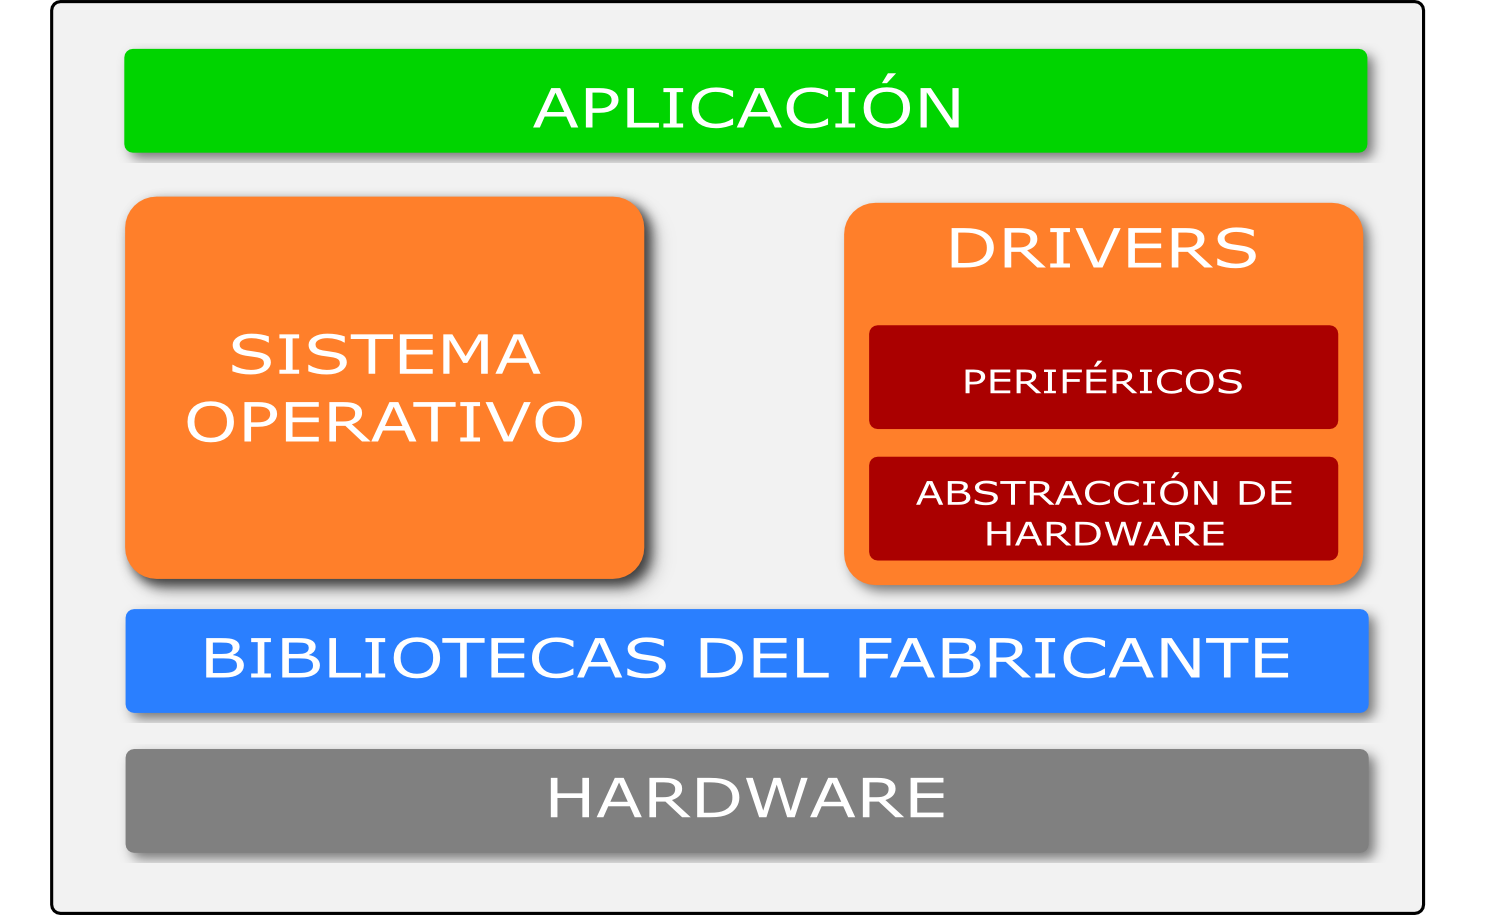
\includegraphics[width=10cm]{./Figures/3_2_2_firmware_diagrama_capas.png}
	\caption{Capas del firmware.}
	\label{fig:firmware_diagrama_capas}
\end{figure}

A continuación se realiza una breve descripción de cada una de las capas:

\begin{itemize}
\item Aplicación. Consiste en el firmware propio del equipo, que utiliza al sistema operativo para implementar la lógica del Smart Plug..
\item Sistema operativo. Consiste en las librerías de FreeOSEK. Como se utilizó un microcontrolador LPC1763 se utilizó la implementación de FreeOSEK para el LPC1769 realizada por Pablo Ridolfi en \citep{repo_ridolfi_freeosek}.
\item Drivers. Dentro de los drivers se encuentras las bibliotecas particulares para controlar tanto los periféricos internos del microcontrolador como los dispositivos externos. La capa de abstracción de hardware, también conocida como HAL (por sus siglas en inglés, Hardware Abstraction Layer), busca generar un nivel más de abstracción entre los drivers de alto nivel y las bibliotecas del fabricante del microcontrolador, lo cual permite, que ante un cambio en el microcontrolador, solamente se deba cambiar la capa HAL.

Para implementar los controladores se utilizó un enfoque orientado a objetos para ordenar las distintas "clases".  Una explicación detallada de este proceso se encuentra en la Subsección \ref{subsec:orientado_a_objetos}.
\item Bibliotecas del fabricante. Son las bibliotecas provistas por NXP para acceder a los periféricos internos del microcontrolador.
\item Hardware. Componentes del Smart Plug.
\end{itemize}

\subsection{Metodología orientada a objetos}
\label{subsec:orientado_a_objetos}

Para implementar los drivers, tanto de los periféricos internos del microcontrolador como de los módulos externos, se decidió implementar una metodología orientada a objetos, a pesar de estar programando en C. La forma de estructurar el código y cada una de las clases surgió a partir de lo explicado por Alex Schreiner en su libro \textit{Object-Oriented Programming With ANSI-C } \citep{schreiner1993}.

Mediante esta forma de programar los drivers se lograron implementar los conceptos de encapsulamiento, polimorfismo y herencia propios de un lenguaje orientado a objetos.

Las clases que se implementaron para este proyecto se pueden ver en el diagrama de clases de la Figura \ref{fig:firmware_diagrama_clases}.

\begin{figure}[h]
	\centering
	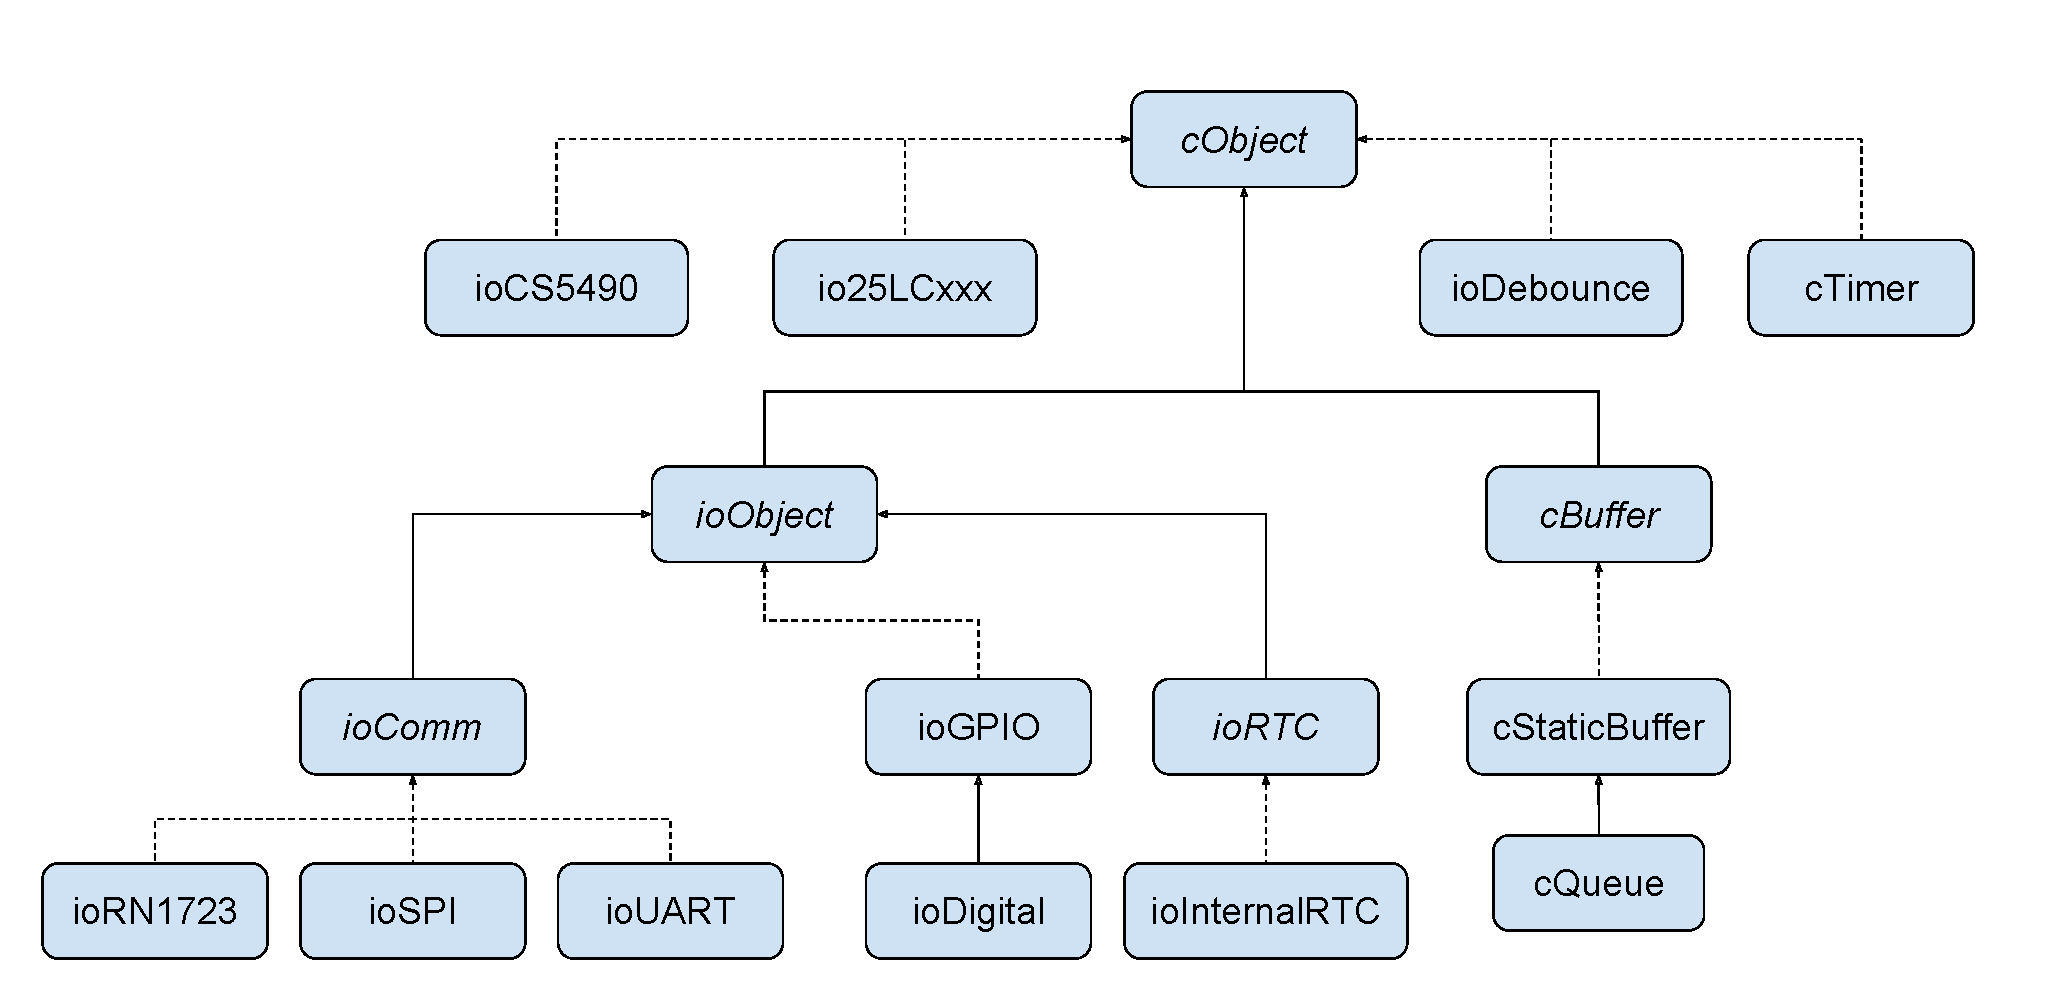
\includegraphics[width=14cm]{./Figures/3_2_3_diagrama-clases-simplificado.pdf}
	\caption{Diagrama de clases de los controladores desarrollados para el firmware.}
	\label{fig:firmware_diagrama_clases}
\end{figure}

La idea general detrás de esta forma para programar módulos de firmware se puede ver en la Figura \ref{fig:firmware_diagrama_interfaces}. Todas las clases implementadas en este trabajo parten de la interfaz \textit{cObject}. Se la llama interfaz y no clase, ya que su comportamiento es similar a las interfaces de Java: \textit{cObject} no implementa la lógica de sus métodos, sino que simplemente declara los prototipos de las funciones (esto se implementa mediante punteros a funciones). Las clases que implementen la interfaz cObject deberán implementar la algoritmia para cada uno de los métodos contenidos en la interfaz \textit{cObject}.

\begin{figure}[h]
	\centering
	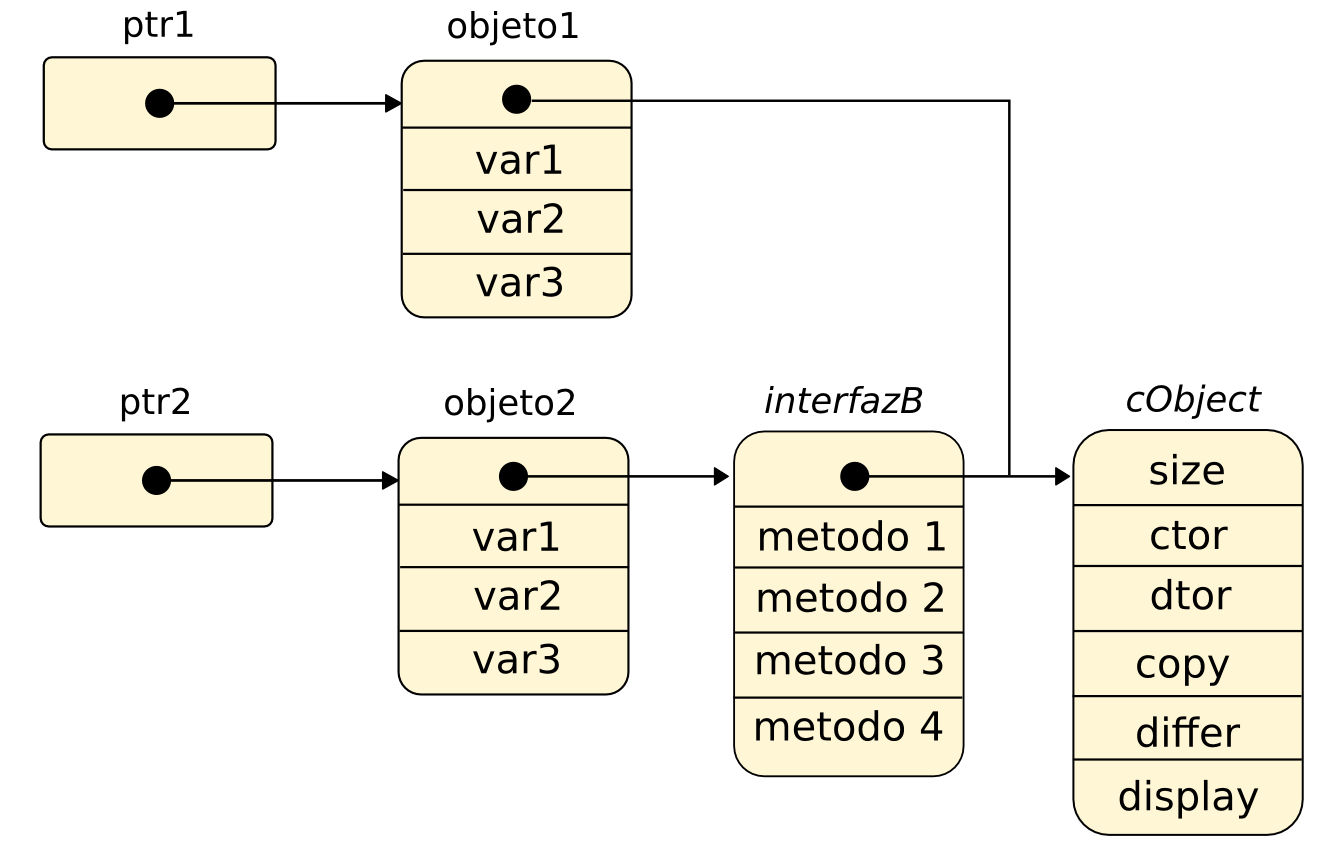
\includegraphics[width=9cm]{./Figures/3_2_3_c_orientado_objetos.png}
	\caption{Creación de interfaces y objetos en C.}
	\label{fig:firmware_diagrama_interfaces}
\end{figure}

Este comportamiento puede verse en la parte superior de la Figura \ref{fig:firmware_diagrama_interfaces}: \textit{objeto1} es una clase que implementa la  interfaz \textit{cObject}. Esta interfaz contiene los métodos básicos necesarios para cualquier otra clase: un constructor, un destructor, una función para crear una copia de un objeto, una función para determinar si dos objetos son iguales y una para mostrar el contenido del objeto de forma comprensible para un humano. Además contiene un campo \textit{size} el cual indica la cantidad de bytes que ocupa una instancia de la clase en memoria RAM.

Por lo tanto \textit{objeto1} debe implementar la lógica de todos los métodos incluidos en \textit{cObject}. Además de implementar la algoritmia, \textit{objeto1} puede contener variables que van a ser propias de cada instancia. En la figura estas serían var1, var2 y var3. Por otro lado, \textit{objeto1} puede declarar funciones que solamente puedan ser utilizadas sobre instancias de la clase \textit{objeto1}.

Finalmente \textit{ptr1} es un puntero a la instancia de \textit{objeto1}. El tipo de variable de \textit{ptr1} es \textit{void*}, es decir que la implementación de la clase queda totalmente encapsulada, ya que la aplicación instancie a \textit{objeto1} no conocerá su estructura interna.

Con esta metodología también es posible implementar la herencia tanto de interfaces como de clases. En la parte inferior de la Figura \ref{fig:firmware_diagrama_interfaces} puede verse un ejemplo de herencia de interfaces. En este caso, la \textit{interfazB} hereda a la interfaz \textit{cObject}, agregando 3 métodos a los ya definidos por \textit{cObject}. Por lo tanto, la clase que implementa la \textit{interfazB} debe implementar todos los métodos, tanto los definidos por \textit{cObject} como los de \textit{interfazB}. En el ejemplo esta clase es \textit{objeto2}, la cual además define 3 variables. Nuevamente \textit{ptr2} es un puntero a \textit{void} el cual apunta al área de memoria donde fue creada la instancia de \textit{objeto2}.

Como puede suponerse esta forma de trabajo requiere además implementar alguna forma de asignación dinámica de memoria. Para este trabajo se decidió implementar un pool de memoria implementado mediante un arreglo de bytes, el cual contiene una sencilla lógica que permite asignar, liberar y unir segmentos continuos (para reducir la fragmentación) del pool de memoria. 

Esta librería es una modificación de la descripta en \citep{an_microchip_malloc}, en la que delante de cada segmento asignado de memoria se coloca un encabezado de dos bytes que indica si está asignado el bloque de memoria o no y la longitud del bloque. El código fuente puede encontrarse dentro de la carpeta \textit{memAlloc} en \citep{repo_firmware}.

Se debe aclarar que esta forma de trabajo no contradice la naturaleza estática del RTOS FreeOSEK. Como condición en la implementación del firmware se estableció que la creación y destrucción de los objetos únicamente se pudiera hacer en el comienzo de la aplicación. De esta forma, cuando el RTOS se encuentra funcionando no se producen más asignaciones dinámicas de memoria y el sistema se comporta como si fuera estático.

En cuanto a las clases desarrolladas se puede mencionar lo siguiente:

\begin{itemize}
\item \textit{ioObject} es una interfaz que hereda a \textit{cObject} y agrega los métodos básicos necesarios para cualquier periférico de entrada/salida: inicialización, habilitación/deshabilitación y escritura/lectura.

\item \textit{ioGPIO} es una clase que implementa a la interfaz \textit{ioObject} y que sirve como base para las clases que describen tipos más específicos de GPIOs, como por ejemplo pines digitales a través de la clase \textit{ioDigital}.

\item \textit{ioDigital} es una clase que herada a \textit{ioGPIO} e implementa la lógica para manejar los GPIO del microcontrolador LPC176x como pines digitales, tanto entradas como salidas.

\item \textit{ioRTC} es una interfaz que hereda a \textit{ioObject} y los métodos básicos necesarios para manejar relojes de tiempo real, tanto internos al microcontrolador, como externos: reset del reloj, lectura y escritura de la hora y fecha.

\item \textit{ioInternalRTC} es una clase que implementa la interfaz \textit{ioRTC} y permite configurar y consultar el RTC interno del microcontrolador LPC176x.

\item \textit{ioComm} es una interfaz que hereda a \textit{ioObject} y agrega los métodos básicos para las clases que modelen periféricos de comunicación: lectura y escritura de cadenas de bytes, determinación de espacio disponible en buffers, habilitación/deshabilitación/consulta de interrupciones.

\item \textit{ioUART} es una clase que implementa la interfaz \textit{ioComm} y que permite manejar las UARTs del microcontrolador LPC176x y las interrupciones relacionadas con estos periféricos. Además agrega el manejo de buffers de recepción y transmisión. La comunicación se puede implementar tanto de forma bloqueante como mediante interrupciones.

\item \textit{ioSPI} es una clase que implementa la interfaz \textit{ioComm} y que permite manejar los SPI del microcontrolador LPC176x. La comunicación es siempre bloqueante.

\item \textit{ioRN1723} es una clase que implementa la interfaz \textit{ioComm} y que permite manejar un módulo WiFi RN1723. Implementa la lógica para poder configurar el módulo, iniciar el modo WPS y AP y manejo de conexiones TCP. Esta clase requiere de otras clases para poder funcionar: \textit{ioUART} para implementar la comunicación con el módulo, \textit{ioDigital} para manejar los pines de reset y algunos GPIO del módulo, \textit{cQueue} para implementar los buffers de recepción y transmisión, \textit{cTimer} para determinar eventos de timeout con el módulo y con las conexiones TCP.

\item \textit{cBuffer} es una interfaz que herada a \textit{cObject} y agrega los métodos necesarios para las clases que modelen contenedores de datos: agregado y borrado de elementos, consulta de elementos, consulta de espacio libre, limpieza del contenedor, etc.

\item \textit{cStaticBuffer} es una clase que implementa la interfaz \textit{cBuffer} y que sirve como base para todas las clases que implementen contenedores de tamaño fijo.

\item \textit{cQueue} es una clase que herera a \textit{cStaticBuffer} e implementa la lógica de una cola, es decir un contenedor de tipo FIFO (First In First Out, primero entra primero sale). Puede contener objetos de cualquier cantidad de bytes pero deben ser todos del mismo tipo.

\item \textit{ioCS5490} es una clase que implementa la interfaz \textit{cObject} que permite manejar el front-end analógico CS5490. Implementa la lógica para poder leer/escribir registros y contiene las variables necesarias para obtener las mediciones eléctricas. Esta clase depende de otras para poder funcionar: \textit{ioUART} para implementar la comunicación con el módulo y \textit{ioDigital} para los pines de reset y de pulsos de energía consumida.

\item \textit{io25LCxxx} es una clase que implementa la interfaz \textit{cObject} que permite manejar memorias EEPROM de la línea 25LC fabricadas por Microchip. Una instancia de esta clase puede ser configurada para escribir/leer/borrar datos de memorias de distintas capacidades, desde 32kbit  hasta 1Mbit. Esta clase depende de \textit{ioSPI} para implementar la comunicación con la memoria externa.

\item \textit{ioDebounce} es una clase que implementa la interfaz \textit{cObject} y permite ejecutar la lógica de un anti-rebote sobre una instancia de la clase \textit{ioDigital}.

\item \textit{ioTimer} es una clase que implementa la interfaz \textit{cObject} y permite implementar timers sencillos y detectar cuando vencen mediante polling. La base de tiempo debe ser establecida por el usuario de la clase \textit{ioTimer}.

\end{itemize}

El código fuente de todas las interfaces y clases puede encontrarse en la carpeta \textit{cObject} en \citep{repo_firmware}. Dentro de esta carpeta también puede encontrarse un diagrama de clases completo (\textit{class\_diag\_cObject.dia}) con los métodos y variables que define cada clase e interfaz.


\subsection{Protocolo de comunicación}
\label{subsection:protocolo}

\begin{figure}[h]
	\centering
	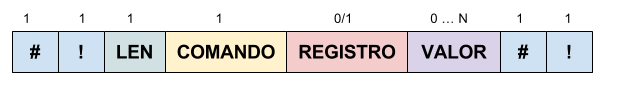
\includegraphics[width=13cm]{./Figures/3_2_4_formato_trama.png}
	\caption{Formato de la trama.}
	\label{fig:formato_trama}
\end{figure}


\subsection{Uso de los comandos}

\begin{figure}[h]
	\centering
	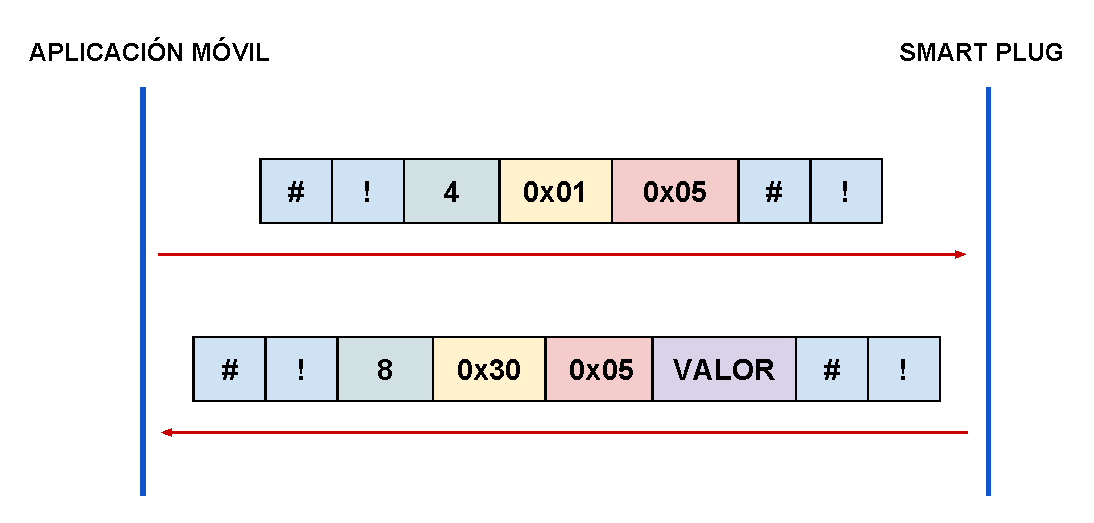
\includegraphics[width=12cm]{./Figures/3_2_5_comunicacion_GET.pdf}
	\caption{Diagrama de comunicación del comando \textit{GET}.}
	\label{fig:comunicacion_get}
\end{figure}


\begin{figure}[h]
	\centering
	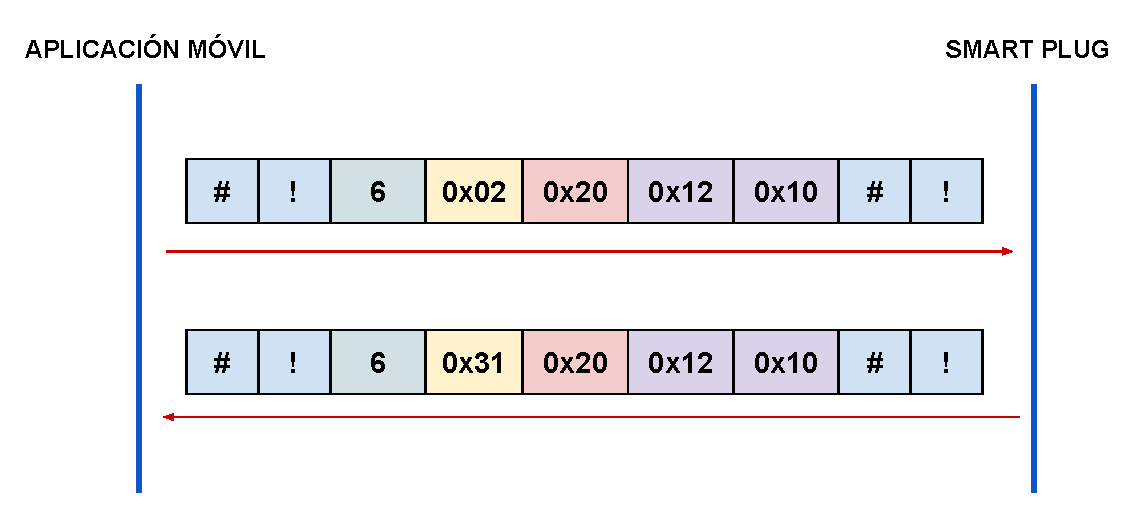
\includegraphics[width=12cm]{./Figures/3_2_5_comunicacion_SET.pdf}
	\caption{Diagrama de comunicación del comando \textit{SET}.}
	\label{fig:comunicacion_set}
\end{figure}


\begin{figure}[h]
	\centering
	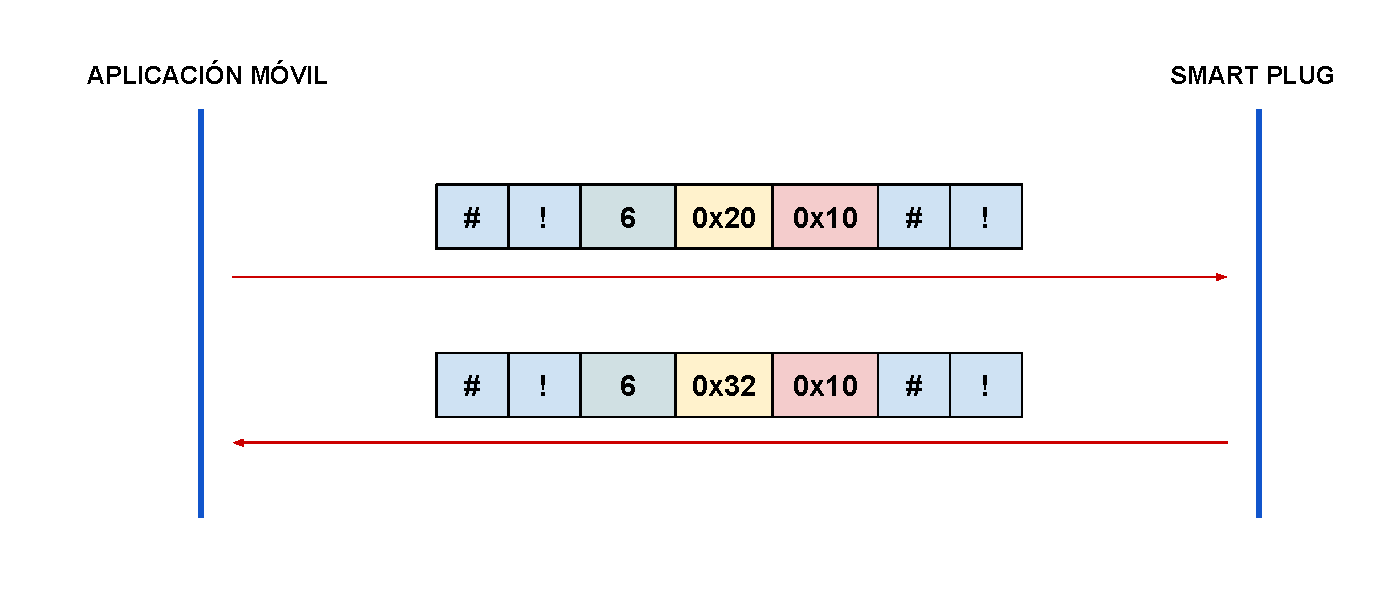
\includegraphics[width=12cm]{./Figures/3_2_5_comunicacion_RESET.pdf}
	\caption{Diagrama de comunicación del comando \textit{RESET}.}
	\label{fig:comunicacion_reset}
\end{figure}


\begin{figure}[h]
	\centering
	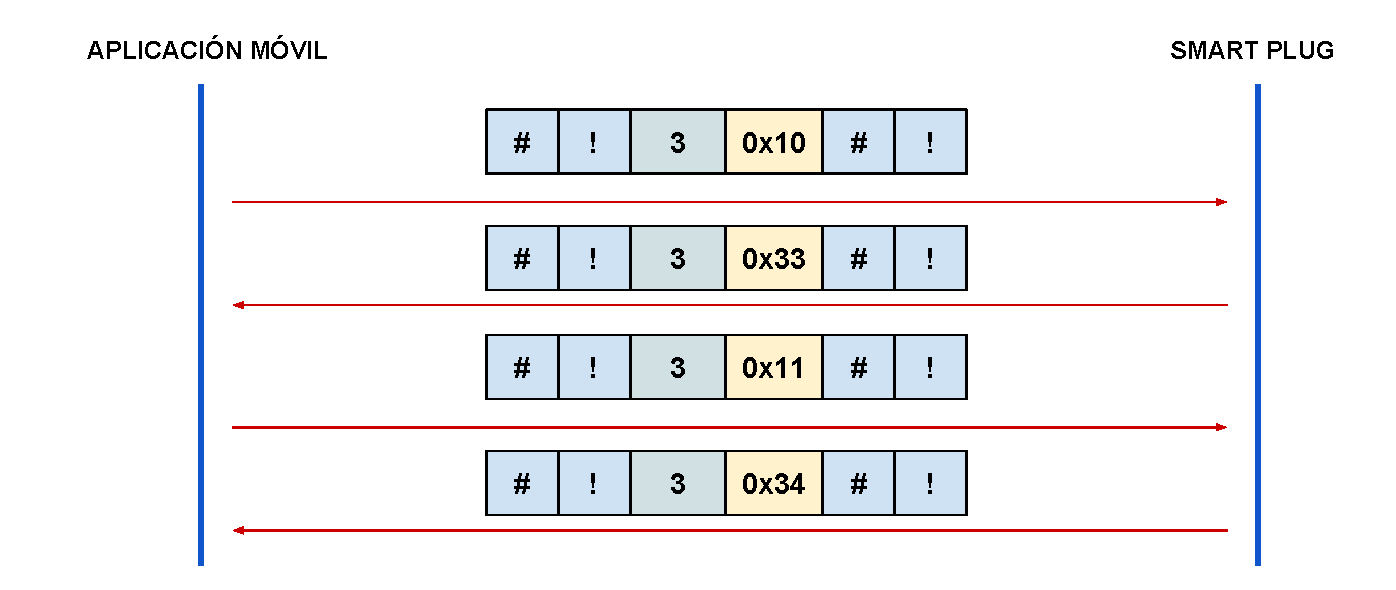
\includegraphics[width=12cm]{./Figures/3_2_5_comunicacion_NODE.pdf}
	\caption{Diagrama de comunicación de los comandos \textit{NODE ON} y \textit{NODE OFF}.}
	\label{fig:comunicacion_node}
\end{figure}


\section{Aplicación Android}
\label{section:app}

\subsection{Maqueta de la aplicación}

\begin{figure}[h]
	\centering
	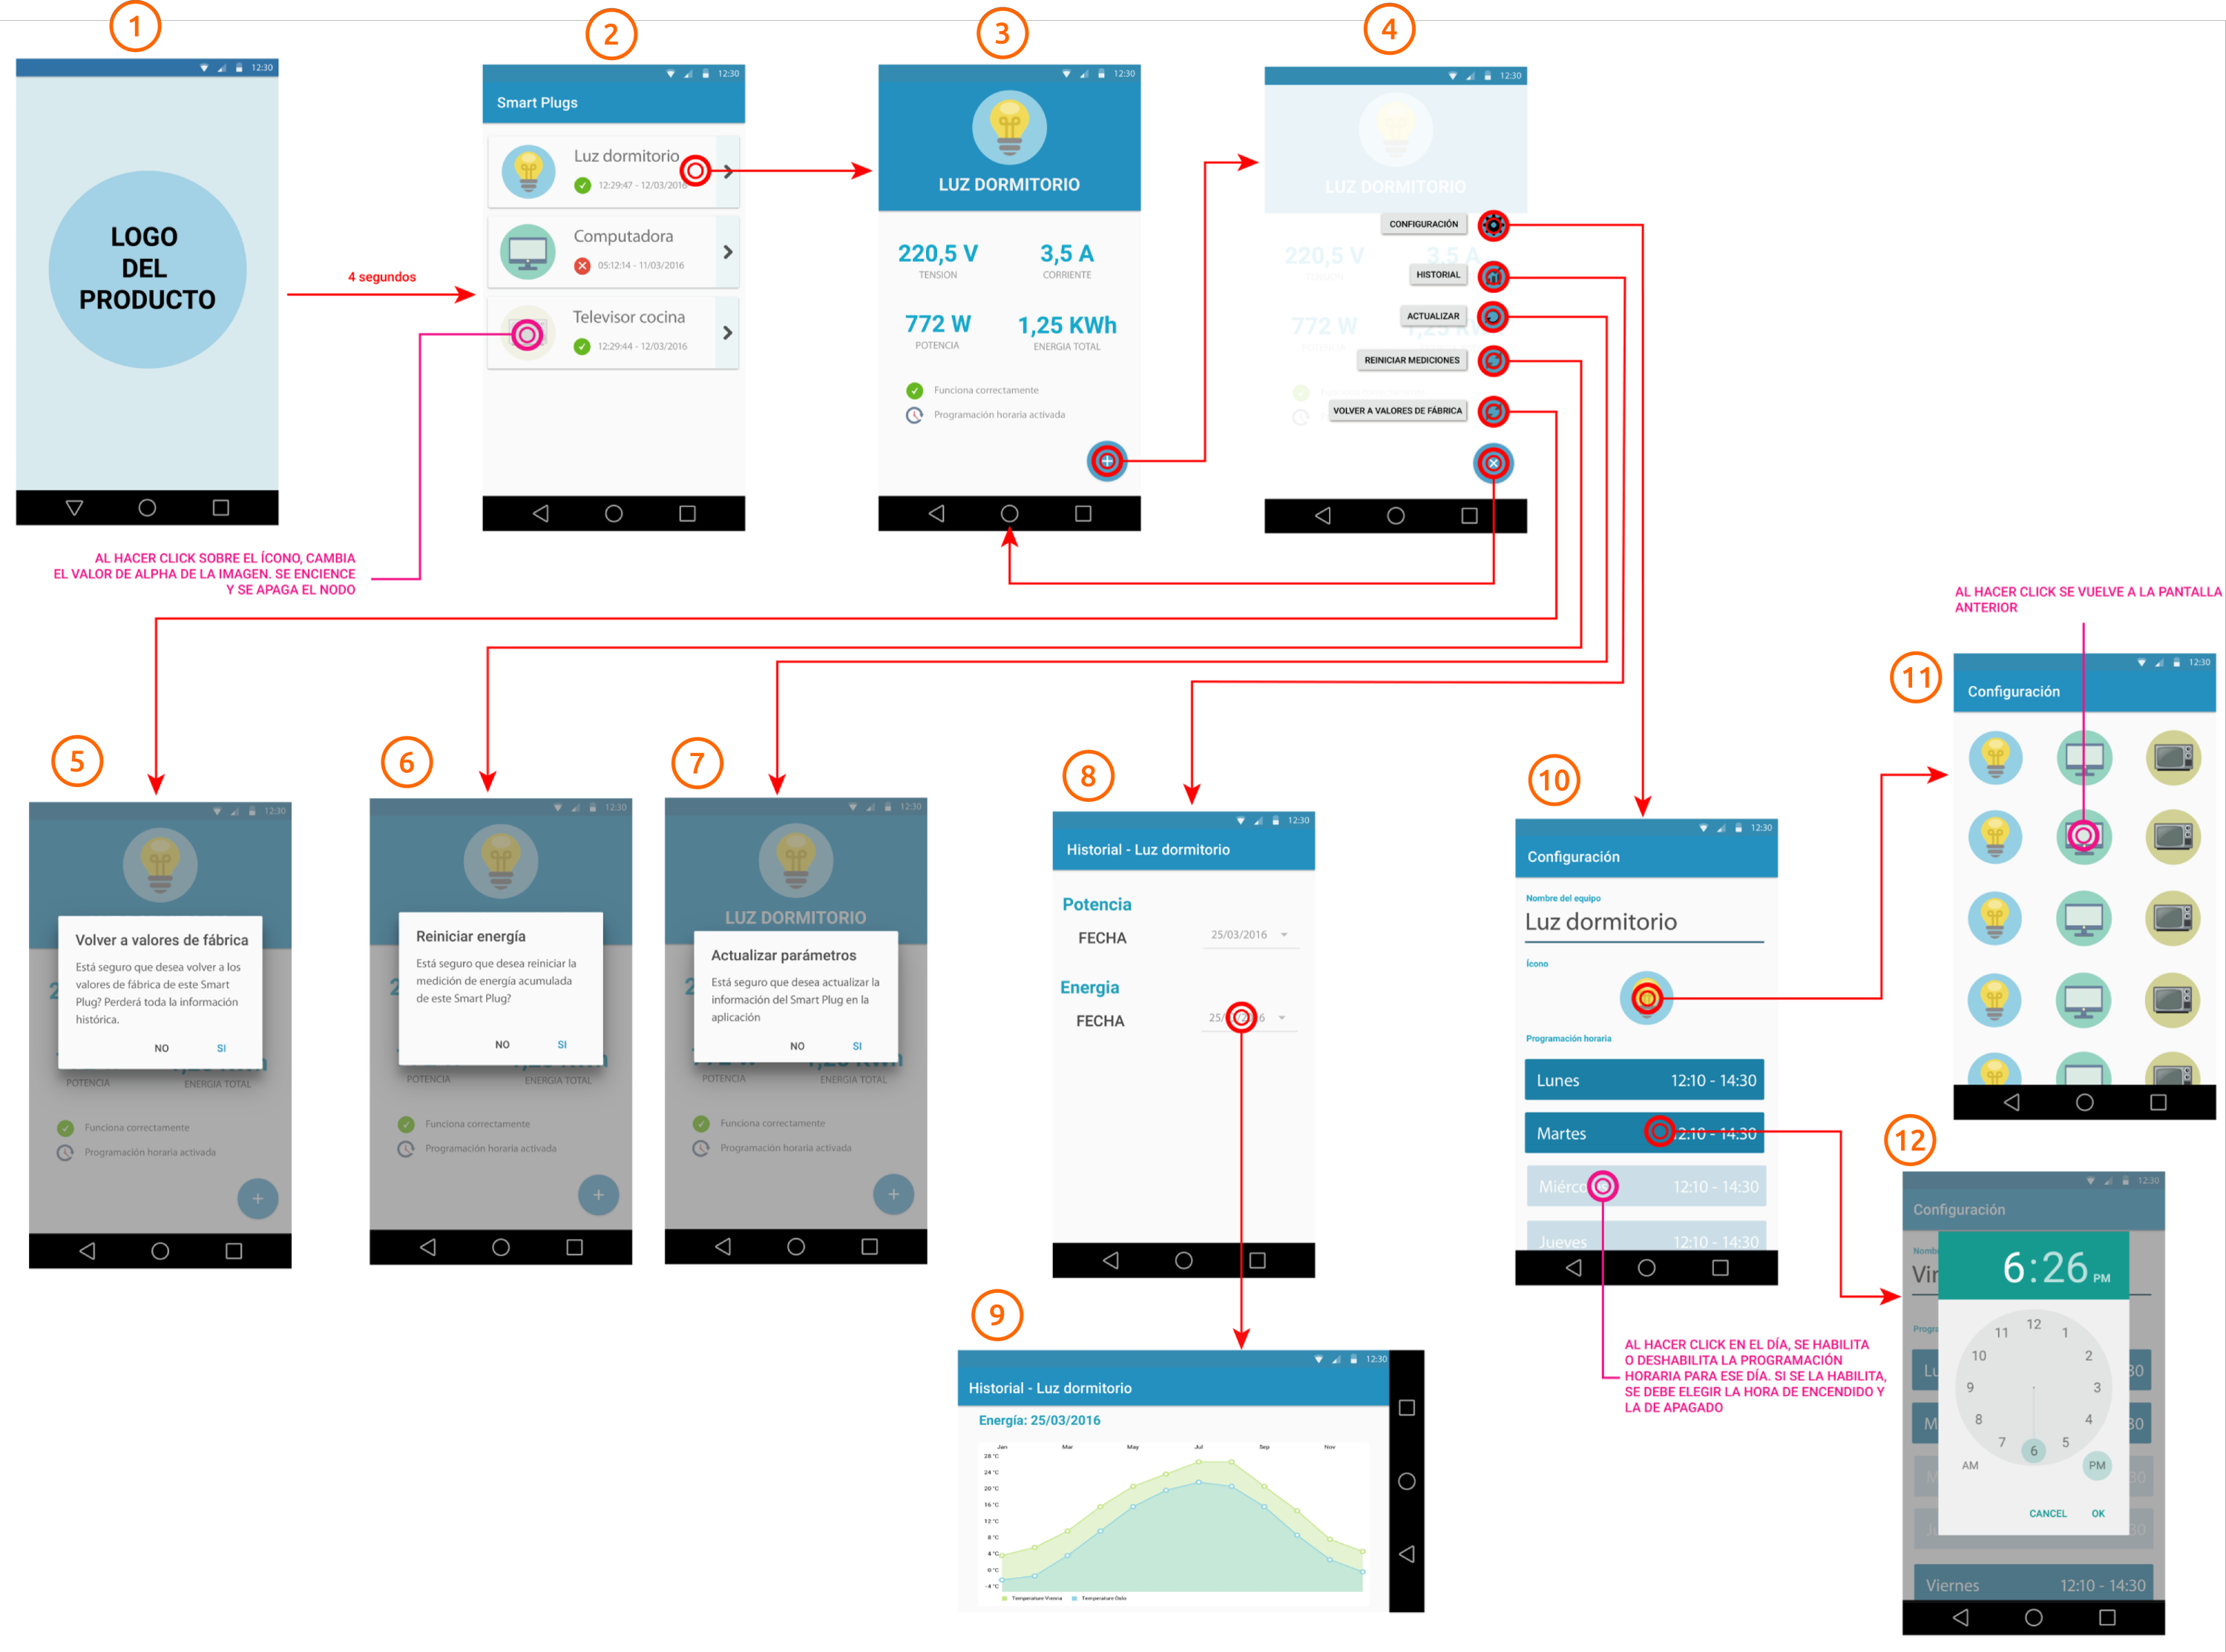
\includegraphics[width=18cm, angle=90]{./Figures/3_3_1_app_wireframe.png}
	\caption{Maqueta de la aplicación móvil.}
	\label{fig:comunicacion_app_wireframe}
\end{figure}


\subsection{Arquitectura de la aplicación}

\begin{figure}[h]
	\centering
	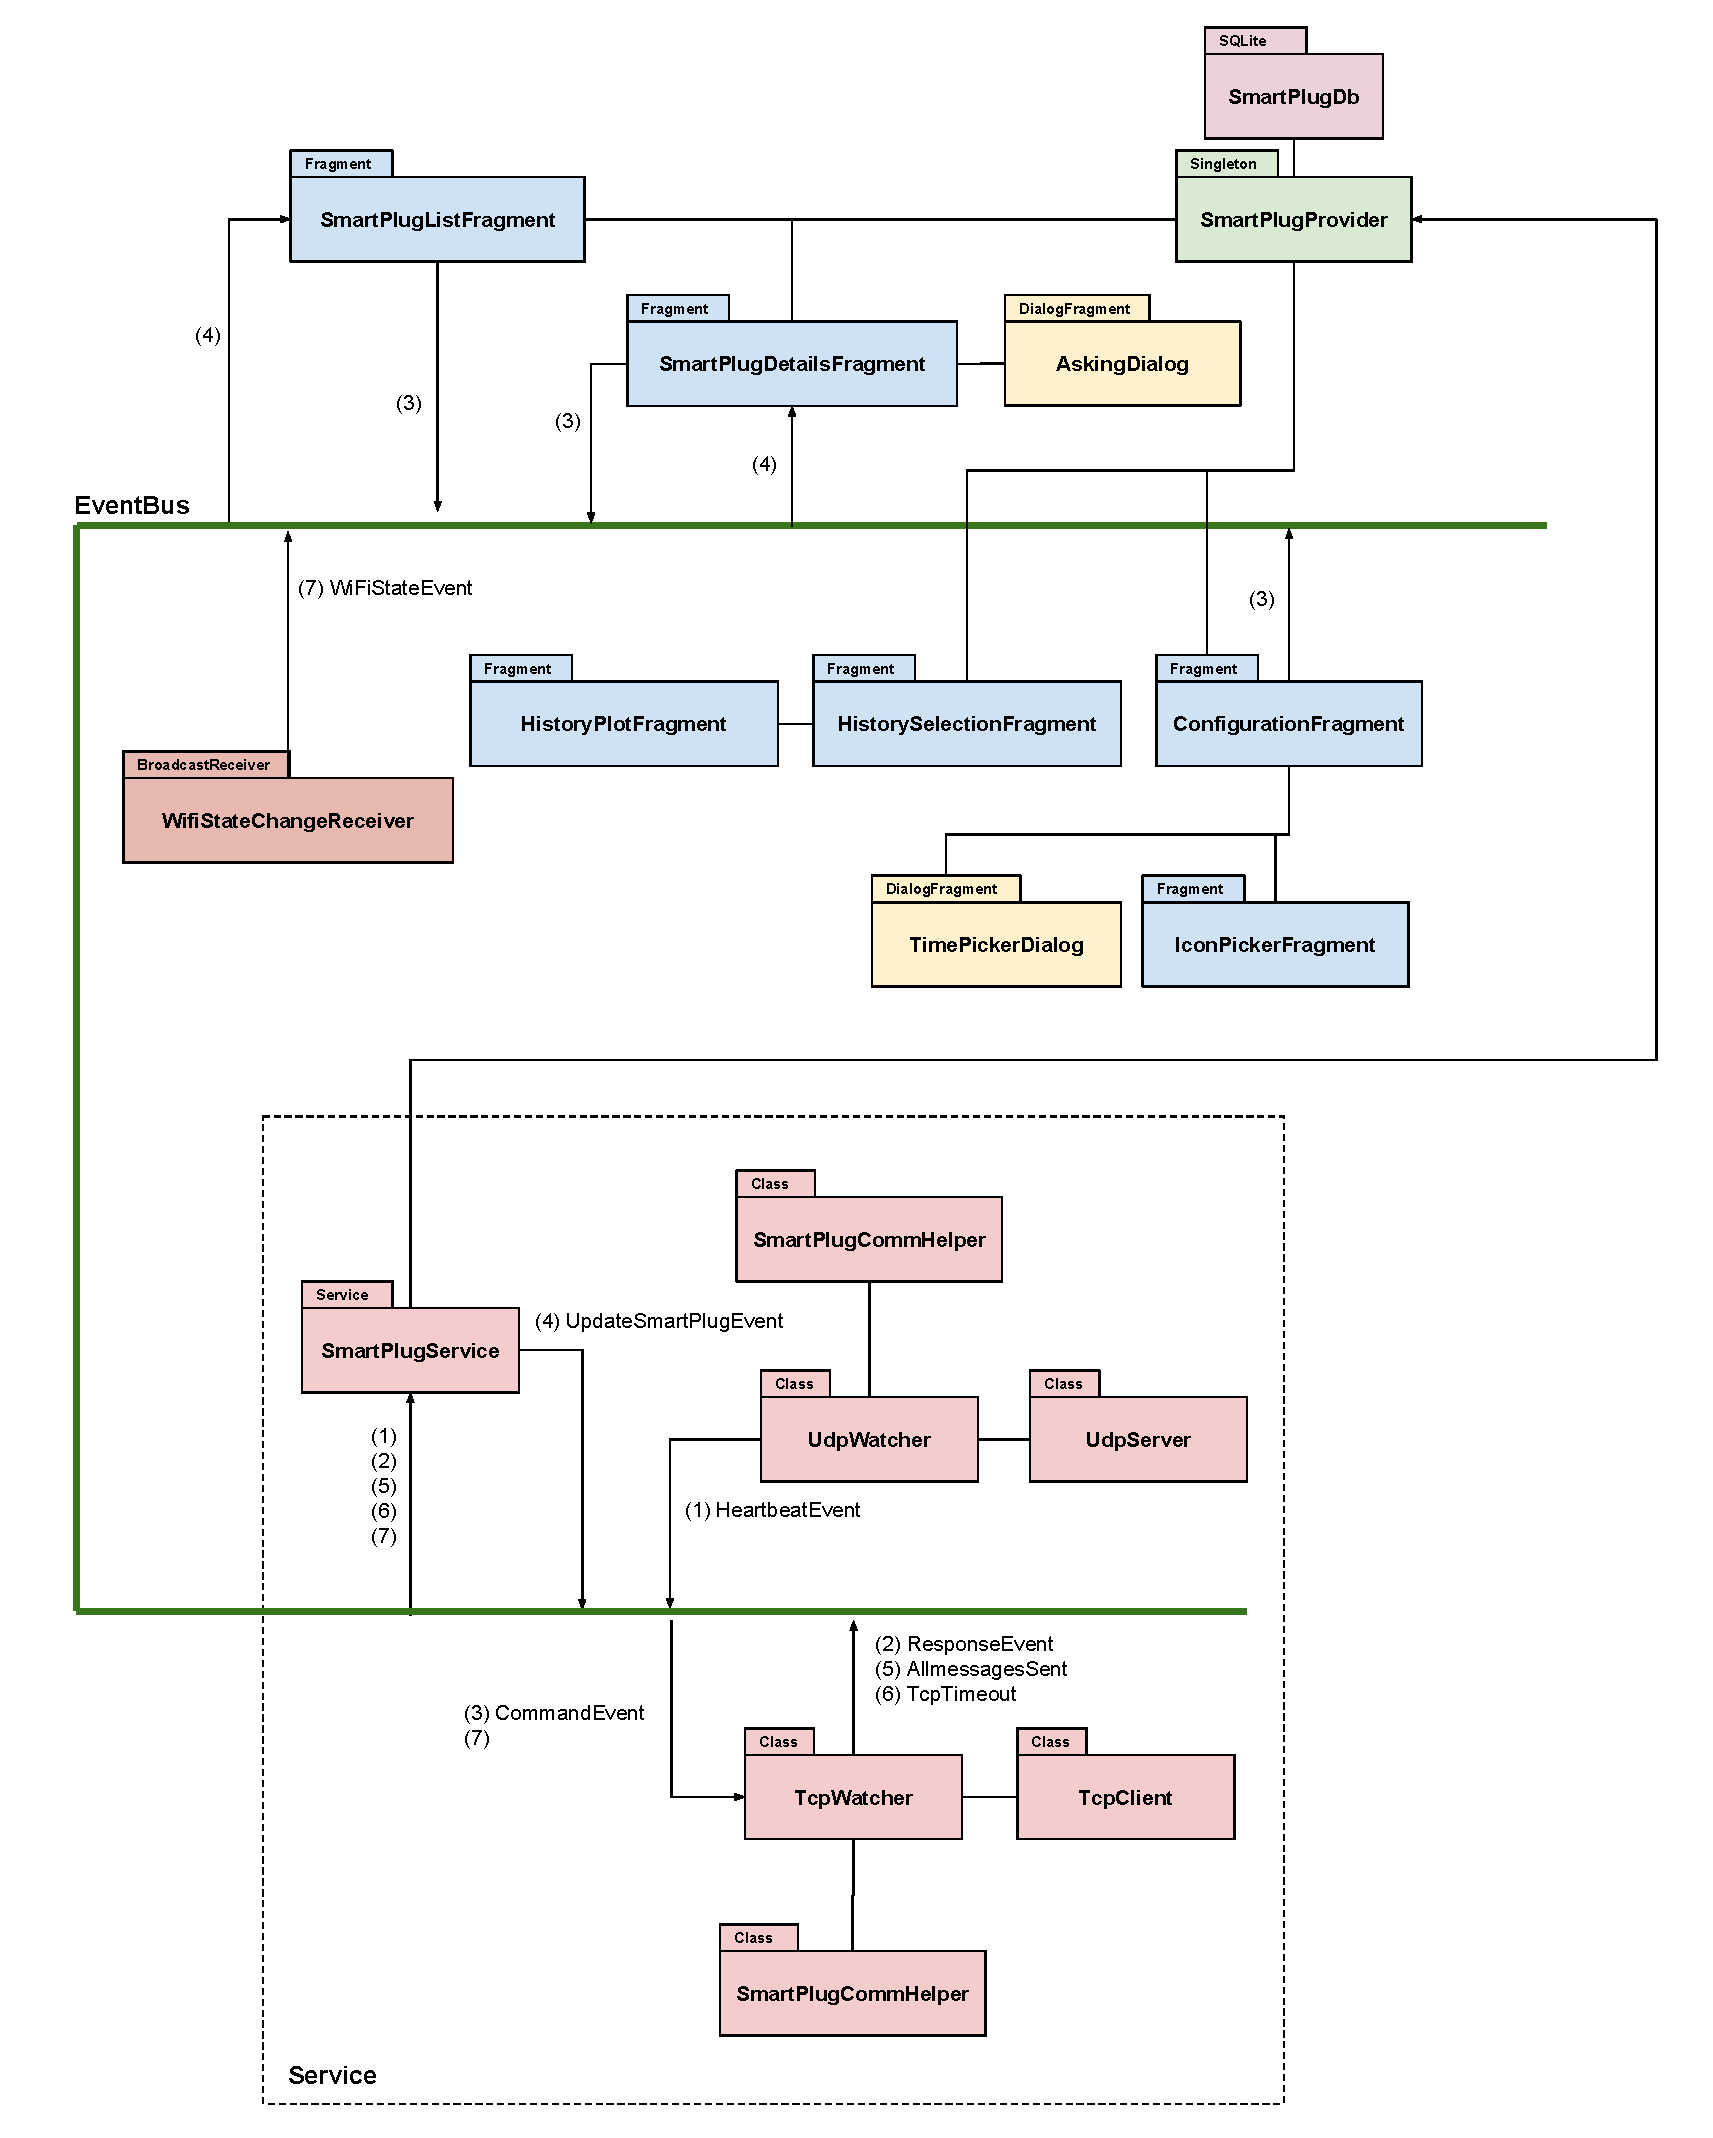
\includegraphics[width=14cm]{./Figures/3_3_2_app-arquitectura.pdf}
	\caption{Relación entre las clases desarrolladas para la aplicación móvil.}
	\label{fig:app_arquitectura}
\end{figure}



